Die nächste Analyse bezieht sich auf das zeitliche Eintreffen von Emails. Durch das Parsen der .pst-Datei lag die Eigenschaft \glqq{}datetime\grqq, welche das Datum und die Zeit der empfangenen E-Mail darstellt in dem Format vor, dass in Abbildung \ref{fig:datetime} zu sehen ist. Mithilfe des Python Codes aus Abbildung \ref{fig:emailsdatetime} werden die Daten in die korrekte Zeitzone konvertiert, weil sie standardmäßig im UTC-Format gespeichert werden. Hierzu wird die Zeitzone erst als UTC deklariert und dann in die gewünschte Zeitzone umgewandelt. Im nachfolgenden Schritt werden die extrahierten Daten als Punktewolke, welche die Ankunftszeiten der E-Mails nach Datum darstellt, geplottet. Dazu werden zwei Spalten mit den Koordinaten der zu verfolgenden Punkte erstellt. Als letzter Schritt wird dann die Punktewolke erstellt. Dazu wurden die Python Bibliotheken \glqq{}matplotlib\grqq{} und \glqq{}seaborn\grqq{} verwendet. In dieser Seminararbeit wurde der vorhandene Datensatz vom Jahr 2020 bis Mitte 2022 analysiert. \newline
Daraus entstand der Graph, der in Abbildung \ref{fig:auswertungzeitlich} abgebildet wird. Klar erkennbar ist hier die Häufung von empfangenen E-Mails zwischen 16 und 18 Uhr. Ebenso ist ab dem Jahr 2022 eine Häufung der Nachrichten im Bereich um 14 bis 15 Uhr erkennbar. Auffällig ist, das zwischen 22 Uhr und 5 Uhr fast keine E-Mails eingetroffen sind. Daraus lässt sich ableiten, dass tatsächlich fast nur Mails gesendet zu Zeiten gesendet werden, bei denen der Nutzer auch selbst aktiv ist. \newline
Die Punktewolke, die sich aus dem zweiten Datensatz ableiten lässt, ist in Abbildung \ref{fig:auswertungzeitlichmerged} zu sehen. Hier ist anzumerken, dass die zeitliche Verteilung leider wenig Aussagekräftig ist, da unter Berücksichtigung aller empfangener E-Mails die hohe Anzahl an Benachrichtigungen von \glqq{}Twitch\grqq{} enthalten ist und diese zu jeder Tages- und Nachtzeit auftreten. Beim herausfiltern all dieser E-Mails waren keine besonderen zeitlichen Auffälligkeiten der anderen Mails erkennbar, da es dafür wiederum zu wenige über den betrachteten Zeitraum waren, wobei dieser sogar schon auf die erste Hälfte des Jahres 2022 eingeschränkt wurde. 

\begin{figure}
    \centering
    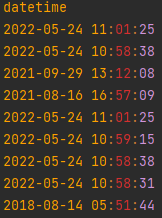
\includegraphics[width=0.50\textwidth]{images/datetime.PNG}
    \caption{E-Mail Eigenschaft datetime} 
    \label{fig:datetime}
\end{figure}

\begin{figure}
    \centering
    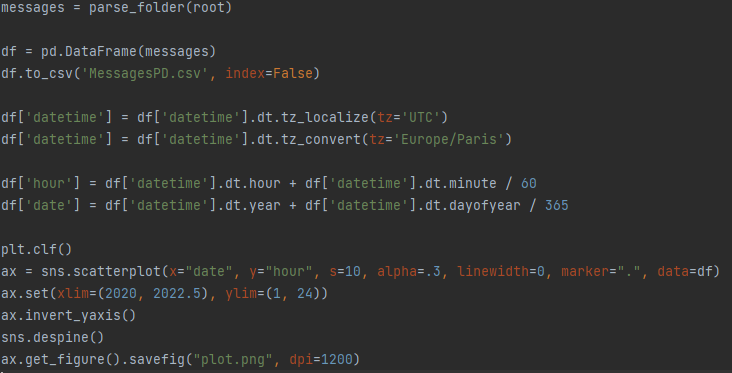
\includegraphics[width=0.75\textwidth]{images/Auswertung_Zeiten.PNG}
    \caption{Python Code - Auswertung hinsichtlich der Empfangszeiten} 
    \label{fig:emailsdatetime}
\end{figure}

\begin{figure}
    \centering
    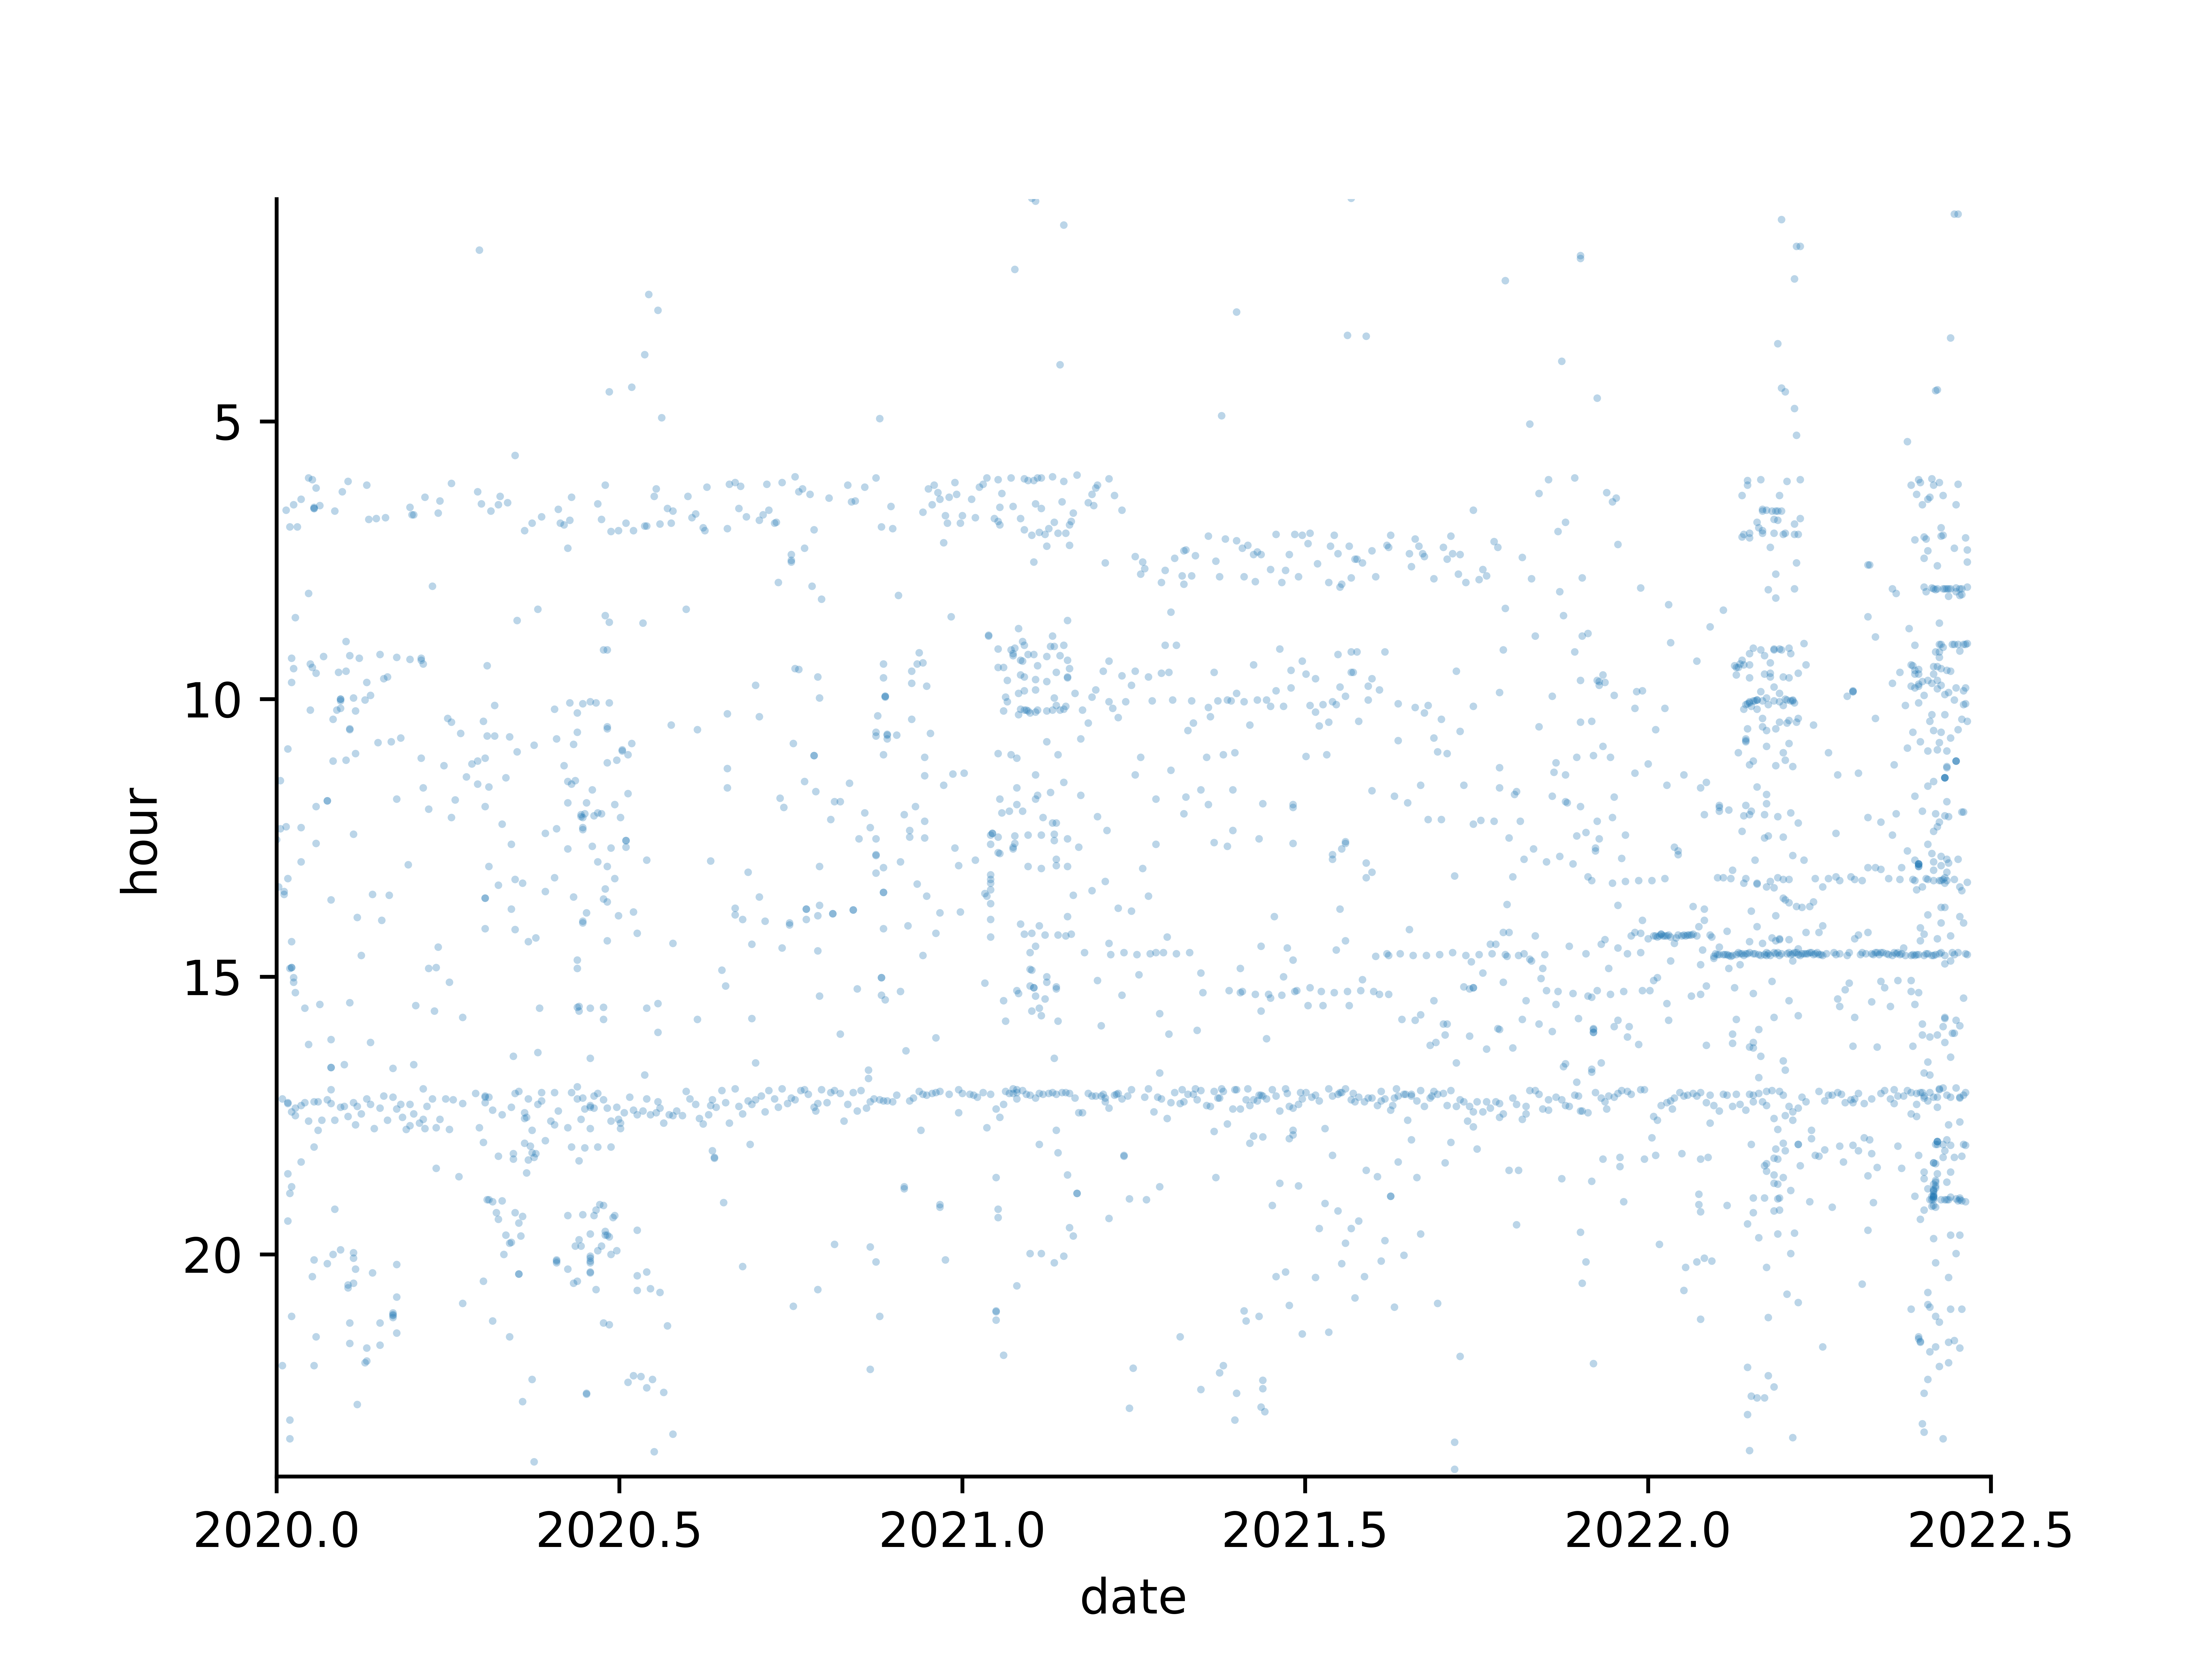
\includegraphics[width=0.75\textwidth]{images/plot.PNG}
    \caption{Zeitliche Verteilung der E-Mails} 
    \label{fig:auswertungzeitlich}
\end{figure}


\begin{figure}
    \centering
    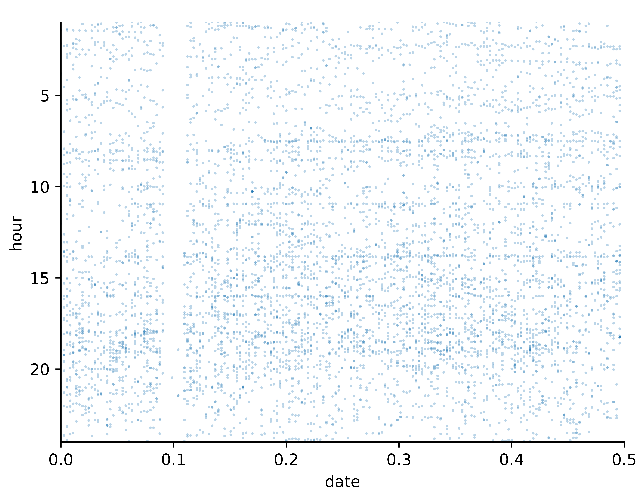
\includegraphics[width=0.75\textwidth]{images/merged_plot.PNG}
    \caption{Zeitliche Verteilung der E-Mails bei zusammengesetztem Postfach} 
    \label{fig:auswertungzeitlichmerged}
\end{figure}